%-------------------------------------------------------------------------------
% seq64_usr_file
%-------------------------------------------------------------------------------
%
% \file        seq64_usr_file.tex
% \library     Documents
% \author      Chris Ahlstrom
% \date        2015-08-31
% \update      2015-11-27
% \version     $Revision$
% \license     $XPC_GPL_LICENSE$
%
%     Provides the usr_file.
%
%-------------------------------------------------------------------------------

\section{Sequencer64 User Configuration File}
\label{sec:seq64_usr_file}

   The \textsl{Sequencer64} configuration file provides a way to give more
   informative names to the MIDI busses, MIDI channels, and MIDI controllers of
   a given system setup.  This configuration will override the default values
   of some drop-down lists and menu items, and make them reflect your names for
   them.

   By default, the list of MIDI items that \textsl{Sequencer64} shows depends
   on one's system setup and whether the manual-alsa-port options is specified
   or not.  Here's our system, which has Timidity installed and running as a
   service, and the manual-alsa-port option turned off, shown in a composite
   view with all menus one can look at for MIDI settings:

\begin{figure}[H]
   \centering 
   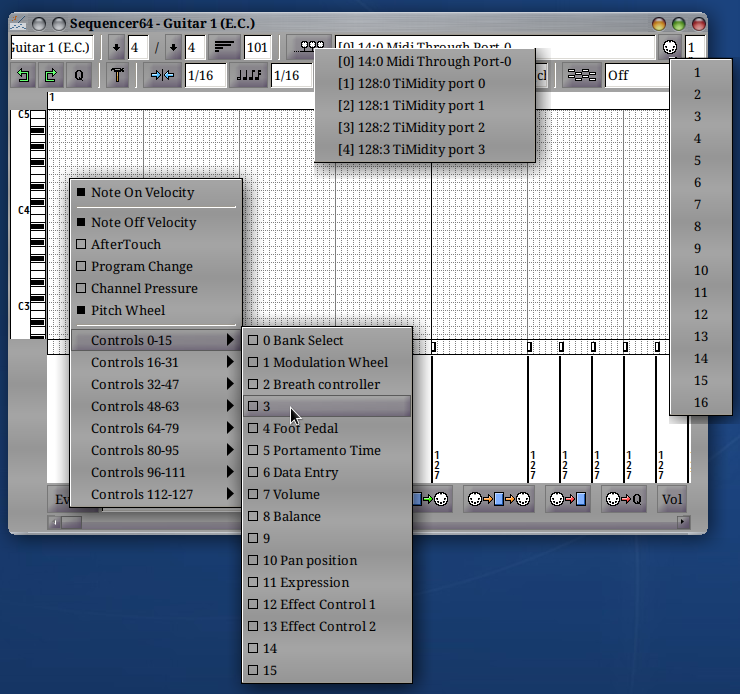
\includegraphics[scale=0.75]{buss/manual-0-buss-dropdown.png}
   \caption{Sequencer64 Composite View of Native Devices}
   \label{fig:seq64_manual_0_buss_dropdown}
\end{figure}

   At the top center, the dropdown menu contains the 5 MIDI busses (also known
   as "MIDI ports") supported by our system.  At right, the MIDI channel shows
   the channels numbers that can be picked for buss 0.  At bottom left, we see
   the default controller values that \textsl{Sequencer64} includes.  We have
   no idea if these correspond to any controllers that the selected MIDI buss
   supports.  We \textsl{can} use this dropdown to see if any such controller
   events are in the loaded MIDI file, of course.

   Now let's assume we have 3 MIDI "buss" devices hooked to our system:
   two Model "2x2" MIDI port devices, and an old PCR-30 MIDI controller
   keyboard.  Let's number them:

   \begin{enumerate}
      \item Model 2x2 A
      \item Model 2x2 B
      \item PCR-30
   \end{enumerate}

   Then assume that we have nine different MIDI instruments in our kit.
   Let's number them, too:

   \begin{enumerate}
      \item Waldorf Micro Q
      \item SuperNova
      \item DrumStation
      \item TX81Z
      \item WaveStation
      \item ESI-2000
      \item ES-1
      \item ER-1
      \item TB-303
   \end{enumerate}

   The Waldorf Micro Q, the SuperNova, and the DrumStation all have a large
   number of special MIDI controller values for affecting the sound they
   produce.  The DrumStation accepts MIDI controllers that change various
   features of the sound of each type of drum it supports.

   The buss devices can be configured (apparently) to route certain
   MIDI channels to certain MIDI devices.  Let's assume we have them
   set up this way:

   \begin{enumerate}
      \item Model 2x2 A
      \begin{itemize}
         \item SuperNova: channels 1 to 8
         \item TX81Z: channels 9 to 11
         \item Waldorf Micro Q: channels 12 to 15
         \item DrumStation: channel 16
      \end{itemize}
      \item Model 2x2 B
      \begin{itemize}
         \item WaveStation: channels 1 to 4
         \item ESI-2000: channels 5 to 14
         \item ES-1: channel 15
         \item ER-1: channel 16
      \end{itemize}
      \item PCR-30
      \begin{itemize}
         \item TB-303: channel 1
      \end{itemize}
   \end{enumerate}

   How can we get \textsl{Sequencer64} to show these items with the proper
   names associated with each device, channel, and controller value?
   We use the oddly-named \textbf{"user" configuration file}.

   \index{sequencer64.usr}
   \index{[sequencer64.usr]}   % for convenience
   The \textsl{Seq24} configuration file was called
   \texttt{.seq24usr}, and it was stored in the user's \texttt{\$HOME}
   directory.
   For \textsl{Sequencer64}, we created an new file-name
   to take its place, with a fall-back to the original file-name if the new
   file does not exist, or if \textsl{Sequencer64} is running in
   legacy mode.

   After you run \textsl{Sequencer64} for the first time, it will generate a
   \texttt{sequencer64.usr} file in your home directory:

   \begin{verbatim}
      /home/ahlstrom/.config/sequencer64/sequencer64.usr
   \end{verbatim}

   It allows you to give an alias to 
   each MIDI bus, MIDI channel, and MIDI control 
   codes, per channel.
   The name is a bit misleading... do not confuse this file with the
   \texttt{sequencer64.rc} file.

   The process for setting up the user file is to:

   \begin{enumber}
      \item Define one or more MIDI busses, the name of each, and what
         instruments are on which channels.  Each buss is configured in a
         section of the form "\textbf{[user-midi-bus-X]}", where "X" ranges
         from 0 on up.
      \item Define all of the instruments and their control-code
         names if they have them.  Each instrument is configured in a
         section of the form "\textbf{[user-instrument-X]}", where "X"
         ranges from 0 on up.
   \end{enumber}

   So, taking our list of devices and channels we created above,
   deducting 1 from each device number and channel number (so that numbering
   starts from 0), and consulting the device manuals to determine the
   controller values it supports, we can assemble a "user" configuration file
   that makes the setup visible in \textsl{Sequencer64}.

   Peruse the next couple of sections to understand a bit about the format of
   this file.  Look at the example file in the \texttt{contrib} directory as
   well, to see the whole thing put together.
   Once you're satisfied, go to
   \sectionref{subsec:seq64_usr_file_midi_bus_results}, and 
   see what it all looks like.

\subsection{Sequencer64 User / MIDI Bus Definitions}
\label{subsec:seq64_usr_file_midi_bus_definitions}

   \index{[user-midi-bus-definitions]}
   This section begins with an
   "INI" group marker \texttt{[user-midi-bus-definitions]}.
   It defines the number of user busses that will be configured in this file.

   \begin{verbatim}
      [user-midi-bus-definitions]
      3     # number of user-defined MIDI busses
   \end{verbatim}

   This means that the \texttt{sequencer64.usr} file will have three MIDI buss
   sections: [user-midi-bus-0], [user-midi-bus-1], and [user-midi-bus-2].
   Here's is an annoted example of one such section:

   \begin{verbatim}
      [user-midi-bus-0]
      2x2 A (SuperNova,Q,TX81Z,DrumStation)     # name of the device
      16                                        # number of channels

      # NOTE: Channels are 0-15, not 1-16.  Instruments set to -1 = GM

      0 1                                       # channel and instrument
      1 1 
      2 1
      3 1
      4 1
      5 1
      6 1
      7 1
      8 3
      9 3
      10 3
      11 0
      12 0
      13 0
      14 0
      15 2
   \end{verbatim}

   Here's an example of one that needs only one override:

   \begin{verbatim}
      [user-midi-bus-2]
      PCR-30 (303)
      1                                         # number of channels
      0 8                                       # channel and instrument
      # The rest default to -1 - General MIDI
   \end{verbatim}

\subsection{Sequencer64 User / MIDI Instrument Definitions}
\label{subsec:seq64_usr_file_midi_instrument_definitions}

   \index{[user-instrument-definitions]}
   This section begins with an
   "INI" group marker \texttt{[user-instrument-definitions]}.
   It defines the number of user instruments that will be configured in this
   file.

   \begin{verbatim}
      [user-instrument-definitions]
      9     # number of user instrument
   \end{verbatim}

   So this "usr" file will define 9 instruments.  We will provide one section
   as a sample.

   \begin{verbatim}
      [user-instrument-0]
      Waldorf Micro Q                     # name of instrument
      128                                 # number of MIDI controllers
      0                                   # first controller value, unnamed
      1 Modulation Wheel
      2 Breath Control
      3 
      4 Foot Control
      5 Glide Rate
      6 
      7 Channel Volume
      8
      9
      10 Pan
      11 
      12 Arp Range (0-9) (1-10 octaves)
      13 Arp Length (0-15) (1-16 steps)
      14 Arp Active (0-3) (Off,On,One Shot,Hold)
      15 LFO 1 Shape (0-5) (Sine,Tri,Square,Saw,Rand,S&H)
         . . .
      119
      120 All Sound Off (0)
      121 Reset All Controllers (0)
      122 Local Control (0-127) (Off,On)
      123 All Notes Off (0)
      124
      125
      126
      127
   \end{verbatim}

   We assume that an unnamed control number is an unsupported control number.

   Here is an instrument where its synthesis parameters can be controlled:

   \begin{verbatim}
      [user-instrument-1]
      SuperNova
      128
      0 Bank Select MSB
      1 Modulation Wheel
      2 Breath Controller
      3 Arp Pattern Select
      4 Ring Modulator 2 * 3 Mix Level
      5 Portamento Time
      6 Data Entry
      7 Part / Program Volume
      8 Effects Confg Morph Amount
      9 Arp Speed (Internal Clock Rate) [*]
      10 Pan
      11 Osc 1 Fine Tune
      12 Osc 3 Fine Tune
      13 Osc 1 Soften
      14 Osc 2 Soften
      15 Osc 3 Soften
      16 LFO 1 Speed
      17 LFO 1 Delay
         . . .
      119 Delay Mod Wheel Depth
      120 All Sound Off
      121 Reset Controllers
      122 Local Control [*]
      123 All Notes Off
      124 All Notes Off
      125 All Notes Off
      126 All Notes Off
      127 All Notes Off
   \end{verbatim}

   Here is an instrument that perhaps has no controllers, or maybe is simply
   not configured yet.

   \begin{verbatim}
      [user-instrument-4]
      WaveStation
      0
   \end{verbatim}

   The sample file \texttt{contrib/scripts/dot-seq24usr} contains examples
   of some other kinds of instruments, such as drum machines.

\subsection{Sequencer64 User / User Interface Settings}
\label{subsec:seq64_usr_file_user_interface_settings}

   \index{[user-interface-settings]}
   This section begins with an
   "INI" group marker \texttt{[user-interface-settings]}.

   It provides for a feature we will hopefully be able to complete some day:
   the better specificiation of the appearance of the user interface.
   Currently, these settings are not yet in force... we still have to figure
   out a fair number of user interface items.

   But, for now, this section shows some of the current values.

   \begin{verbatim}

      #   ======== Sequencer64-Specific Variables Section ========

      [user-interface-settings]

      # These settings specify the soon-to-be-modifiable sizes of
      # the Sequencer64 user-interface elements.

      # Specifies the style of the main-window grid of patterns.
      # 0 = normal style, matches the GTK theme, has brackets.
      # 1 = white grid boxes that have brackets.
      # 2 = black grid boxes.
      2       # grid_style

      # Specifies box style box around a main-window grid of patterns.
      # 0  = Draw a whole box around the pattern slot.
      # 1  = Draw brackets on the sides of the pattern slot.
      # 2 and up = make the brackets thicker and thicker.
      # -1 = same as 0, draw a box one-pixel thick.
      # -2 and lower = draw a box, thicker and thicker.
      2       # grid_brackets

      # Specifies the number of rows in the main window.
      # At present, only a value of 4 is supportable.
      # In the future, we hope to support an alternate value of 8.
      4       # mainwnd_rows

      # Specifies the number of columns in the main window.
      # At present, only a value of 8 is supportable.
      8       # mainwnd_cols

      # Specifies the maximum number of sets, which defaults to 1024.
      # It is currently never necessary to change this value.
      32      # max_sets

      # Specifies the border width in the main window.
      0      # mainwid_border

      # Specifies the border spacing in the main window.
      2      # mainwid_spacing

      # Specifies some quantity, it is not known what it means.
      0      # control_height

      # Specifies the initial zoom for the piano rolls.  Ranges from 1.
      # to 32, and defaults to 2 unless changed here.

      2      # zoom

      # Specifies if the key, scale, and background sequence are to be
      # applied to all sequences, or to individual sequences.  The
      # behavior of Seq24 was to apply them to all sequences.  But
      # Sequencer64 takes it further by applying it immediately, and
      # by saving to the end of the MIDI file.  Note that these three
      # values are stored in the MIDI file, not this configuration file.
      # Also note that reading MIDI files not created with this feature
      # will pick up this feature if active, and the file gets saved.
      # It is contagious.
      #
      # 0 = Allow each sequence to have its own key/scale/background.
      #     Settings are saved with each sequence.
      # 1 = Apply these settings globally (similar to seq24).
      #     Settings are saved in the global final section of the file.

      1      # global_seq_feature

      # Specifies if the old, console-style font, or the new anti-
      # aliased font, is to be used as the font throughout the GUI.
      # In legacy mode, the old font is the default.
      #
      # 0 = Use the old-style font.
      # 1 = Use the new-style font.

      1      # use_new_font

      # Specifies if the user-interface will support two song editor
      # windows being shown at the same time.  This makes it easier to
      # edit songs with a large number of sequences.
      #
      # 0 = Allow only one song editor (performance editor).
      # 1 = Allow two song editors.

      1      # allow_two_perfedits

      # Specifies the number of 4-measure blocks for horizontal page
      # scrolling in the song editor.  The old default, 1, is a bit
      # small.  The new default is 4.  The legal range is 1 to 6, where
      # 6 is the width of the whole performance piano roll view.

      4      # perf_h_page_increment

      # Specifies the number of 1-track blocks for vertical page
      # scrolling in the song editor.  The old default, 1, is a bit
      # small.  The new default is 8.  The legal range is 1 to 18, where
      # 18 is about the height of the whole performance piano roll view.

      8      # perf_v_page_increment
   \end{verbatim}

\subsection{Sequencer64 User / User MIDI Settings}
\label{subsec:seq64_usr_file_user_midi_settings}

   \index{[user-midi-settings]}
   This section begins with an
   "INI" group marker \texttt{[user-midi-settings]}.

   It provides for a feature we will hopefully be able to complete some day:
   Being able to support files with different PPQN properly, and to specify the
   global defaults for tempo, beats per measure, and so on.

   \begin{verbatim}
      [user-instrument-4]
      [user-midi-settings]

      # These settings specify MIDI-specific value that might be
      # better off as variables, rather than constants.
      # Specifies parts-per-quarter note to use, if the MIDI file.
      # does not override it.  Default is 192, but we'd like to go
      # higher than that.  BEWARE:  STILL GETTING IT TO WORK!
      192       # midi_ppqn

      # Specifies the default beats per measure, or beats per bar.
      # The default value is 4.
      4       # midi_beats_per_measure/bar

      # Specifies the default beats per minute.  The default value
      # is 120, and the legal range is 20 to 500.
      120       # midi_beats_per_minute

      # Specifies the default beat width. The default value is 4.
      4       # midi_beat_width

      # Specifies the buss-number override. The default value is -1,
      # which means that there is no buss override.  If a value
      # from 0 to 31 is given, then that buss value overrides all
      # buss values specified in all sequences/patterns.
      # Change this value from -1 only if you want to use a single
      # output buss, either for testing or convenience.  And don't
      # save the MIDI afterwards, unless you really want to change
      # all of its buss values.
      -1      # midi_buss_override
   \end{verbatim}

\subsection{Sequencer64 User / Results}
\label{subsec:seq64_usr_file_midi_bus_results}

   Okay, now we have this file copied to our home directory:

   \begin{verbatim}
      /home/ahlstrom/.config/sequencer64/sequencer64.usr
   \end{verbatim}

   If we'd already run \textsl{Sequencer64} at least once, we'd have
   overwritten the skeleton sample file that \textsl{Sequencer64}
   writes by default.  We now have a full-fledged "user" file.

   However, because we don't actually have all that equipment (we got the
   example from the Web, for cryin' out loud), let's see what we end up with
   when we run \textsl{Sequencer64} this time.

\begin{figure}[H]
   \centering 
   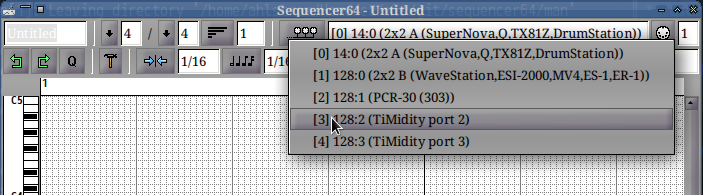
\includegraphics[scale=0.75]{buss/manual-0-userfile-buss-dropdown.png}
   \caption{Sequencer64 Composite View of Non-Native Devices}
   \label{fig:seq64_manual_0_userfile_buss_dropdown}
\end{figure}

   Compare that diagram to \figureref{fig:seq64_manual_0_buss_dropdown}.
   If the original figure, we saw the 5 native busses (ports) on our system,
   their bare-bones channel numbers, and the default controller values.  In
   this new figure, we see the three buss devices (ports), plus the two
   Timidity ports.  If we stopped the Timidity service, these would go away.

   Look at the selected buss, "[0]".  It's 16 channels are now associated with
   the devices to which the channels have been assigned.

   Thus, when we have a new pattern we've created in \textsl{Sequencer64},
   can assign it to exactly the buss and device we want.

   If we don't have port-mappers installed, and thus have only one playback
   device plugged into the buss, we can still create a setup that
   shows the device and a specific program setup.  Doing so would be tedious,
   but perhaps there's some automated way to do it?

   Lastly, note the following figure.

\begin{figure}[H]
   \centering 
   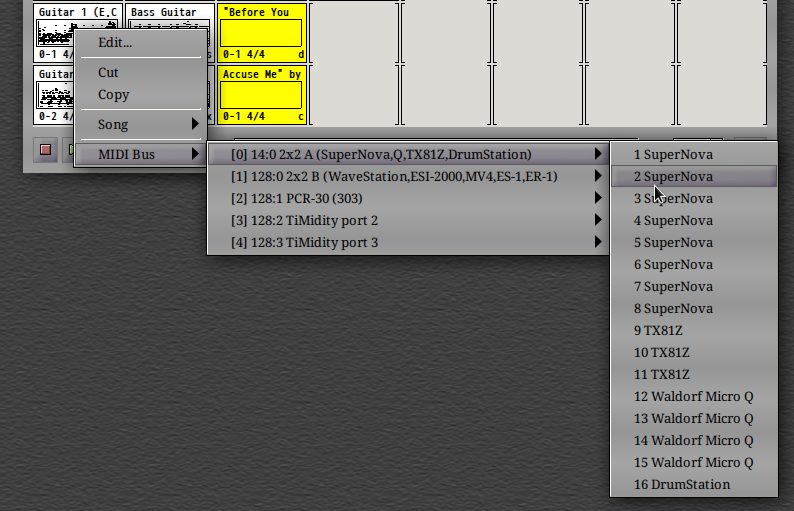
\includegraphics[scale=0.75]{buss/manual-0-userfile-seq-buss-dropdowns.png}
   \caption{The MIDI Bus Menu for a Specific Pattern}
   \label{fig:seq64_manual_0_userfile_seq_buss_dropdown}
\end{figure}

   This figure shows that we can also select the desired port and channel
   directly from the main window.

   There's a lot more to the "user" configuration file than we've exposed here,
   but finding more information about this file has proven a bit tricky.

   Sometime we would like to create a "user" that sets up the
   \textsl{Yoshimi} 1.3.5+ software synthesizer as a device and instrument.

%-------------------------------------------------------------------------------
% vim: ts=3 sw=3 et ft=tex
%-------------------------------------------------------------------------------
